% DISC-IP-003  (JMFK)
% Invention disclosure: variable projection fitting of dark adaptation
% recovery curves in the RapiDA dark adaptometer.
% Compile with xelatex. Figure files fig1-model-curve.tex,
% fig2-varpro-loop.tex, fig3-grid-search.tex must sit alongside this file.
\documentclass[11pt,a4paper]{article}
\usepackage[margin=25mm]{geometry}
\usepackage{iftex}
\ifpdftex
  \usepackage[T1]{fontenc}
  \usepackage[utf8]{inputenc}
  \usepackage{helvet} % closest stock match to Helvetica Neue under pdflatex
\else
  \usepackage{fontspec}
  \IfFontExistsTF{Helvetica Neue}
    {\setmainfont{Helvetica Neue}}
    {\relax} % fall back to the default font if Helvetica Neue is absent
\fi
\usepackage{amsmath}
\usepackage{tikz}
\usetikzlibrary{positioning, arrows.meta}
\usepackage{pgfplots}
\pgfplotsset{compat=1.18}
\usepackage{booktabs}
\usepackage{fancyhdr}
\usepackage[framemethod=tikz]{mdframed}
\usepackage{pdfpages}
\usepackage{enumitem}
\usepackage{natbib} % Loads the natbib package


% -- figure colour definitions (required by all three figures) --
\definecolor{coneC}{HTML}{D85A30}
\definecolor{rodC}{HTML}{534AB7}
\definecolor{tealC}{HTML}{0F6E56}
\definecolor{grayC}{HTML}{5F5E5A}

% -- document identity --
\newcommand{\docid}{DISC-IP-003}
\newcommand{\docversion}{v0.6 draft}
\newcommand{\docdate}{21 August 2026}

% -- headers and footers --
\pagestyle{fancy}
\fancyhf{}
\fancyhead[L]{\small MuMac Ltd}
\fancyhead[R]{\small \docid\ \docversion}
\fancyfoot[L]{\footnotesize Confidential: prepared for the purpose of
  obtaining legal advice}
\fancyfoot[R]{\small Page \thepage}
\renewcommand{\headrulewidth}{0.4pt}

% -- placeholder box for content to be completed --
\newmdenv[linecolor=coneC, linewidth=1pt, roundcorner=4pt,
  backgroundcolor=coneC!6, frametitle={To complete before submission},
  frametitlefont=\small\bfseries]{todo}
  
  

\begin{document}

% ================= title block =================
\begin{center}
{\LARGE Invention disclosure}\\[2mm]
{\Large Variable projection fitting of dark adaptation\\
recovery curves}\\[6mm]
\begin{tabular}{ll}
\toprule
Document ID & \docid \\
Version & \docversion \\
Date & \docdate \\
Author & JMFK \\
Company & MuMac Ltd \\
Status & Draft for review \\
\bottomrule
\end{tabular}
\end{center}

\vspace{4mm}
\noindent\textbf{Version history}

\noindent\begin{tabular}{llll}
\toprule
Version & Date & Author & Change \\
\midrule
v0.1 & 13 August 2026 & JMFK & Initial draft \\
v0.2 & 14 August 2026 & JMFK & Novelty basis, disclosure record,\\
     &                &      & reduction to practice, grid bounds \\
v0.3 & 14 August 2026 & JMFK & Market context (WP); Appendix A\\
     &                &      & (knitted R Markdown) incorporated \\
v0.4 & 19 August 2026 & JMFK & Validation experiment completed;\\
     &                &      & alpha flag reworded; grid spec\\
     &                &      & aligned to implementation \\
v0.5 & 21 August 2026 & JMFK & Cross-platform determinism\\
     &                &      & confirmed on RISC-V; Appendix~A\\
     &                &      & determinism section evidenced \\
v0.6 & 21 August 2026 & JMFK & Inventor's granted patent added as\\
     &                &      & prior art with distinguishing\\
     &                &      & discussion; early-termination claim\\
     &                &      & withdrawn and attributed \\
\bottomrule
\end{tabular}

\vspace{6mm}
\section{Document purpose and scope}
This document describes a method for fitting dark adaptation recovery
curves, as implemented in the RapiDA dark adaptometer, and will be used to 
seek advice on patentability. It is intended for MuMac's patent attorney
and, in abridged form, for the MuMac board. This document and its contents
are confidential.

\section{Background}
Dark adaptation, the recovery of visual sensitivity after exposure to a
bright light, is a functional biomarker for age-related macular
degeneration (AMD). Rod-mediated recovery is measurably delayed in early
AMD, often before structural changes are visible, which makes the shape of
the recovery curve clinically valuable for early detection \cite{Jackson:2014aa}.

The RapiDA dark adaptometer measures this recovery. The participant is
exposed to a controlled bleach and their detection threshold is then
sampled repeatedly in darkness. The clinical output is not the raw
thresholds but the parameters of a model fitted to them; the quality,
speed, and repeatability of that fit determine the quality of the device's
output.

\section{The model}
We model the recovery of visual sensitivity during dark adaptation with
the function
\begin{equation}
\text{thres}(t) = ct + cc\,e^{-t/\tau} + S2\,(t-\alpha)\,H(t-\alpha),
\label{eq:model}
\end{equation}
where:
\begin{itemize}[nosep]
\item $\text{thres}(t)$ is the measured threshold at time $t$ after bleach;
\item $ct$ is the cone threshold, the plateau to which cone-mediated
  sensitivity recovers;
\item $cc$ is the cone coefficient, the amplitude of the cone recovery
  component;
\item $\tau$ is the cone time constant;
\item $S2$ is the slope of the second (rod-mediated) component of
  recovery;
\item $\alpha$ is the rod-cone break, the time at which rod recovery
  begins;
\item $H(t-\alpha)$ is the Heaviside step function, equal to $0$ for
  $t < \alpha$ and $1$ for $t \geq \alpha$.
\end{itemize}
The term $(t-\alpha)H(t-\alpha)$ is therefore a ramp: it is zero before
the rod-cone break and changes linearly with slope $S2$ after it.
Figure~\ref{fig:model} shows the model and its components.

\begin{figure}[ht]
\centering
% fig1-model-curve.tex  (JMFK)
% Dark adaptation model: cone branch, cone threshold ct, rod branch from alpha.
% Requires: tikz, pgfplots (\pgfplotsset{compat=1.18}), arrows.meta.
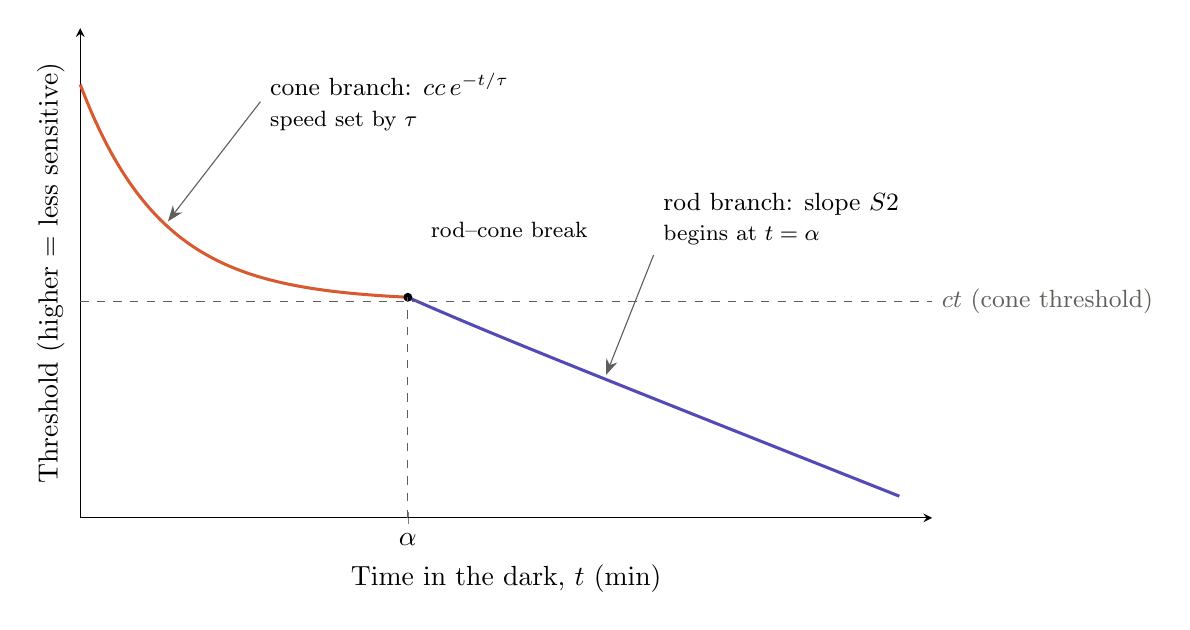
\begin{tikzpicture}
% ---- model parameters: edit these, everything else follows ----
\def\pCT{1.0}      % cone threshold
\def\pCC{1.0}      % cone coefficient
\def\pTAU{2.5}     % cone time constant (min)
\def\pALPHA{10}    % rod-cone break (min)
\def\pSTWO{-0.06}  % rod slope (negative = threshold falls)
\def\pTMAX{25}     % end of plotted time range (min)
% ---- callout layout: x positions of the two arrow targets ----
\def\xConePt{2.6}
\def\xRodPt{16}
% ---- derived quantities (do not edit) ----
\pgfmathsetmacro{\yBreak}{\pCT + \pCC*exp(-\pALPHA/\pTAU)}
\pgfmathsetmacro{\yConePt}{\pCT + \pCC*exp(-\xConePt/\pTAU)}
\pgfmathsetmacro{\yRodPt}{\pCT + \pCC*exp(-\xRodPt/\pTAU) + \pSTWO*(\xRodPt-\pALPHA)}
\pgfmathsetmacro{\yMax}{(\pCT + \pCC)*1.13}
\pgfmathsetmacro{\xMax}{\pTMAX + 1}
\begin{axis}[
  width=124mm, height=78mm,
  axis lines=left,
  xlabel={Time in the dark, $t$ (min)},
  ylabel={Threshold (higher $=$ less sensitive)},
  xmin=0, xmax=\xMax, ymin=0, ymax=\yMax,
  ytick=\empty,
  xtick={\pALPHA}, xticklabels={$\alpha$},
  clip=false,
  every axis plot/.append style={line width=1.1pt},
]
% cone-dominated portion (full model, rod term zero before alpha)
\addplot[coneC, domain=0:\pALPHA, samples=120]
  {\pCT + \pCC*exp(-x/\pTAU)};
% rod-dominated portion (full model including the ramp)
\addplot[rodC, domain=\pALPHA:\pTMAX, samples=120]
  {\pCT + \pCC*exp(-x/\pTAU) + \pSTWO*(x-\pALPHA)};
% rod-cone break marker
\fill (axis cs:\pALPHA,\yBreak) circle[radius=1.6pt];
% ct plateau guide
\draw[dashed, grayC] (axis cs:0,\pCT) -- (axis cs:\xMax,\pCT)
  node[anchor=west, font=\small] {$ct$ (cone threshold)};
% alpha guide
\draw[dashed, grayC] (axis cs:\pALPHA,0) -- (axis cs:\pALPHA,\yBreak);
\node[anchor=west, font=\footnotesize]
  at (axis cs:{\pALPHA+0.4},{\yBreak+0.31}) {rod--cone break};
% cone branch callout
\node[anchor=west, font=\small, align=left] (conelbl)
  at (axis cs:{0.55*\pALPHA},{0.85*\yMax})
  {cone branch: $cc\,e^{-t/\tau}$\\ \footnotesize speed set by $\tau$};
\draw[grayC, shorten >=1.5pt, -{Stealth[length=2mm]}]
  (conelbl.west) -- (axis cs:\xConePt,\yConePt);
% rod branch callout
\node[anchor=west, font=\small, align=left] (rodlbl)
  at (axis cs:{\pALPHA+7.5},{0.61*\yMax})
  {rod branch: slope $S2$\\ \footnotesize begins at $t=\alpha$};
\draw[grayC, shorten >=1.5pt, -{Stealth[length=2mm]}]
  (rodlbl.south west) -- (axis cs:\xRodPt,\yRodPt);
\end{axis}
\end{tikzpicture}

\caption{The dark adaptation model. The cone branch (orange) decays with
time constant $\tau$ towards the cone threshold $ct$; at the rod-cone
break $\alpha$ the rod branch (purple) begins, changing with slope $S2$.
Parameter values are illustrative.}
\label{fig:model}
\end{figure}

\section{The problem with conventional fitting}
Equation~\eqref{eq:model} has five unknown parameters. The conventional
approach is to estimate all five simultaneously by iterative nonlinear
least squares. This has three practical defects for a clinical device:
\begin{enumerate}[nosep]
\item \textbf{Starting guesses.} Iterative solvers require initial values
  for all five parameters. Poor guesses cause failed or wrong fits, and
  choosing good guesses on noisy clinical data is itself unsolved.
\item \textbf{Local minima.} The five-dimensional error surface has
  multiple minima. The solver can converge to a plausible-looking but
  wrong answer, and there is no internal signal that it has done so.
\item \textbf{Irreproducibility.} Different starting guesses, solver
  settings, or library versions can produce different fitted parameters
  from identical data. For a medical device this is a regulatory and
  repeatability problem, not merely an inconvenience.
\end{enumerate}
These concerns are not hypothetical. MuMac's current instruments produce
real-time parameter estimates during the test using gradient descent, and
a single fit can require up to 20{,}000 iterations. The iteration count
is data-dependent and unbounded in principle, which makes worst-case
timing on device hardware difficult to guarantee.

\section{The method}
\subsection{Rewriting the model in a familiar form}
Most STEM scientists are familiar with the equation of a straight line,
\begin{equation}
y = c + mx,
\end{equation}
where $y$ is the response, $x$ is the independent variable, $c$ is the
intercept and $m$ is the gradient. Fitting this line to data by ordinary
least squares (OLS) has a closed-form solution: no iteration, no starting
guesses.

Our aim is to show that, under one condition, our model has exactly the
same character. We want to reach the form
\begin{equation}
\mathbf{Y} = a + \mathbf{B}\,\mathbf{F}(\mathbf{x}),
\end{equation}
where $\mathbf{Y}$ is the vector of participant responses, $\mathbf{x}$ is
the vector of response time stamps, $a$ is an intercept, $\mathbf{F}$ is a
set of basis functions evaluated at those time stamps, and $\mathbf{B}$ is
a vector of coefficients. This is the straight-line equation with the
single term $mx$ replaced by a sum of curved terms.

Suppose the two nonlinear parameters, $\tau$ and $\alpha$, are held fixed.
Then define two basis functions:
\begin{equation}
f_1(\mathbf{x}) = e^{-\mathbf{x}/\tau}, \qquad
f_2(\mathbf{x}) = (\mathbf{x}-\alpha)\,H(\mathbf{x}-\alpha).
\end{equation}
The model becomes
\begin{equation}
\mathbf{Y} = ct + cc\,f_1(\mathbf{x}) + S2\,f_2(\mathbf{x})
           = a + \mathbf{B}\,\mathbf{F}(\mathbf{x}),
\end{equation}
with $a = ct$ playing the role of the intercept $c$, and
$\mathbf{B} = (cc,\ S2)$. This is a linear model. Every quantity we do not
know appears only as an intercept or a multiplying coefficient. Those
familiar with OLS will recognise that the best-fitting $a$ and
$\mathbf{B}$ can be computed together in closed form, exactly as for the
straight line.

\subsection{The variable projection loop}
The full model is nonlinear only through $\tau$ and $\alpha$. Variable
projection (VarPro) exploits this structure:
\begin{enumerate}[nosep]
\item For any candidate pair $(\tau, \alpha)$, the intercept and
  coefficients $(ct, cc, S2)$ are obtained analytically by least squares.
  They are never searched for.
\item The optimisation therefore reduces from a five-parameter nonlinear
  search to a two-parameter search over $(\tau, \alpha)$ alone.
\end{enumerate}
Figure~\ref{fig:loop} shows the loop.

\begin{figure}[ht]
\centering
% fig2-varpro-loop.tex  (JMFK)
% Variable projection search loop: only (tau, alpha) is searched;
% ct, cc, S2 are solved in closed form at every candidate.
% Requires: tikz with libraries positioning, arrows.meta.
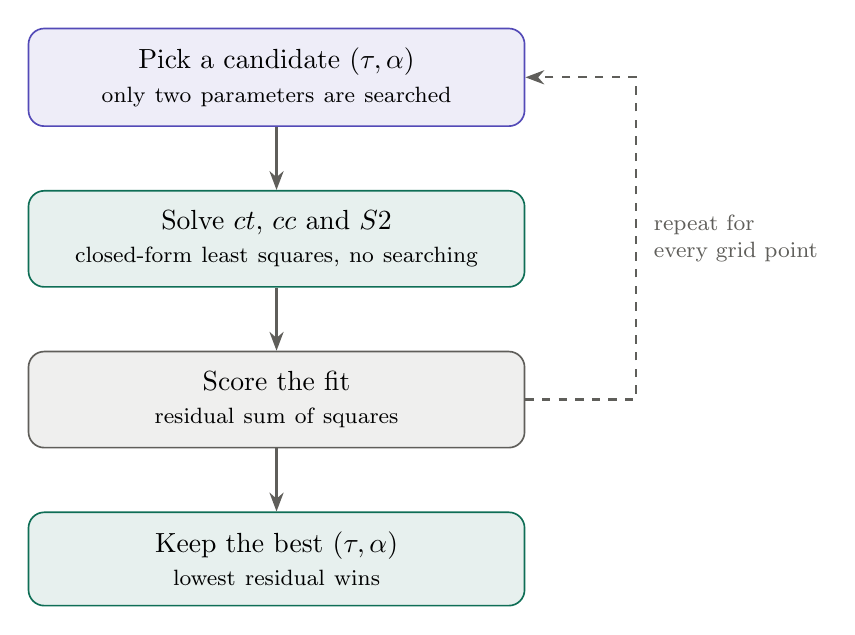
\begin{tikzpicture}[
  node distance=8mm,
  box/.style={rectangle, rounded corners=2mm, draw, line width=0.6pt,
              text width=58mm, align=center, inner sep=2.5mm},
  searched/.style={box, draw=rodC, fill=rodC!10},
  solved/.style={box, draw=tealC, fill=tealC!10},
  neutral/.style={box, draw=grayC, fill=grayC!10},
  arr/.style={-{Stealth[length=2.4mm]}, line width=0.8pt, grayC},
]
\node[searched] (pick)
  {Pick a candidate $(\tau,\alpha)$\\ \footnotesize only two parameters are searched};
\node[solved, below=of pick] (solve)
  {Solve $ct$, $cc$ and $S2$\\ \footnotesize closed-form least squares, no searching};
\node[neutral, below=of solve] (score)
  {Score the fit\\ \footnotesize residual sum of squares};
\node[solved, below=of score] (keep)
  {Keep the best $(\tau,\alpha)$\\ \footnotesize lowest residual wins};
\draw[arr] (pick) -- (solve);
\draw[arr] (solve) -- (score);
\draw[arr] (score) -- (keep);
% return path of the outer loop
\draw[arr, dashed] (score.east) -- ++(14mm,0) |- (pick.east)
  node[pos=0.25, right, font=\footnotesize, align=left, xshift=1mm]
  {repeat for\\ every grid point};
\end{tikzpicture}

\caption{The variable projection search loop. Only the two nonlinear
parameters $(\tau,\alpha)$ are searched (purple); the intercept and
coefficients $(ct, cc, S2)$ are obtained analytically at every candidate
(teal).}
\label{fig:loop}
\end{figure}

Because the two-dimensional $(\tau,\alpha)$ space is small, it can be
searched exhaustively over a grid (Figure~\ref{fig:grid}). Every cell of
the grid costs a single closed-form solve, so the entire space is
evaluated, the global minimum over the grid is found by construction, and
identical data always produce identical fitted parameters.

\begin{figure}[ht]
\centering
% fig3-grid-search.tex  (JMFK)
% Exhaustive grid search over the (tau, alpha) plane. Cell shade = fit error
% (darker = better); the star marks the lowest residual. Every cell costs one
% closed-form solve, so the search is deterministic and reproducible.
% Requires: tikz with library arrows.meta. Shading is synthetic/illustrative.
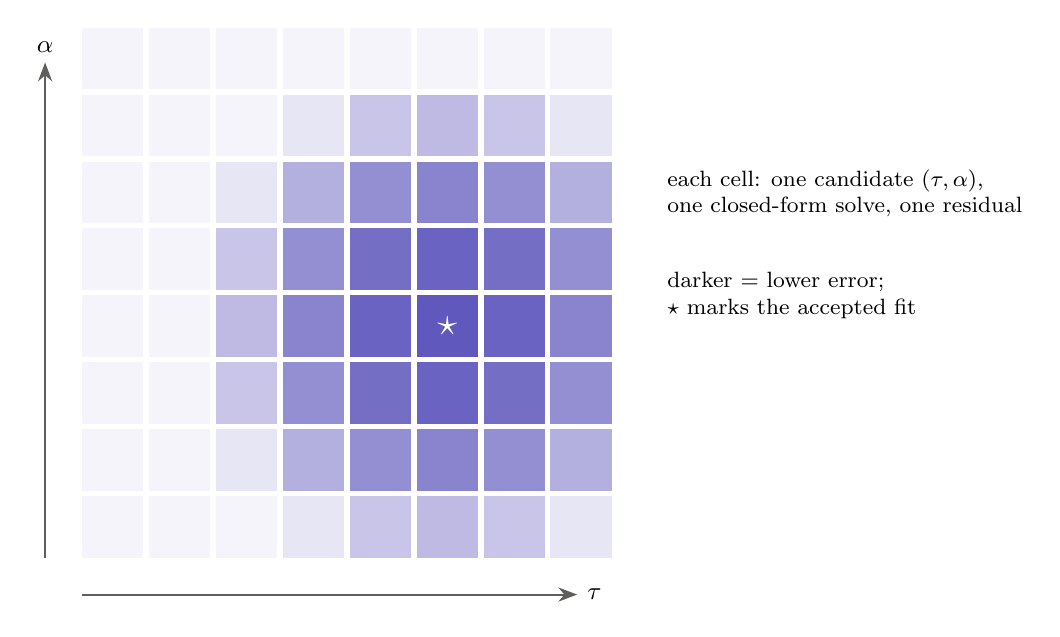
\begin{tikzpicture}[x=8.5mm, y=8.5mm]
% ---- grid parameters: edit these, everything else follows ----
\def\gN{8}          % grid is gN x gN cells
\def\gBestTau{5}    % column of the best cell (0-based)
\def\gBestAlpha{3}  % row of the best cell (0-based)
\def\gShadeMax{92}  % shade percentage at the minimum (darkest)
\def\gShadeSlope{6.0} % how fast shade fades with error distance
\def\gShadeMin{6}   % shade floor at the grid edges (lightest)
% ---- derived quantities (do not edit) ----
\pgfmathtruncatemacro{\gLast}{\gN - 1}
\pgfmathsetmacro{\gAxisEnd}{\gN - 0.6}
\foreach \i in {0,...,\gLast}{
  \foreach \j in {0,...,\gLast}{
    \pgfmathsetmacro{\err}{(\i-\gBestTau)*(\i-\gBestTau)
                         + (\j-\gBestAlpha)*(\j-\gBestAlpha)}
    \pgfmathsetmacro{\pct}{max(\gShadeMin, \gShadeMax - \gShadeSlope*\err)}
    \fill[rodC!\pct] (\i, \j) rectangle ++(0.92, 0.92);
  }
}
% best cell
\node[white, font=\Large\bfseries]
  at ({\gBestTau+0.46}, {\gBestAlpha+0.46}) {$\star$};
% axes
\draw[-{Stealth[length=2.4mm]}, grayC, line width=0.7pt]
  (0,-0.55) -- (\gAxisEnd,-0.55) node[right, font=\small, black] {$\tau$};
\draw[-{Stealth[length=2.4mm]}, grayC, line width=0.7pt]
  (-0.55,0) -- (-0.55,\gAxisEnd) node[above, font=\small, black] {$\alpha$};
% legend
\node[anchor=west, font=\footnotesize, align=left]
  at ({\gN+0.6}, {0.68*\gN})
  {each cell: one candidate $(\tau,\alpha)$,\\ one closed-form solve, one residual};
\node[anchor=west, font=\footnotesize, align=left]
  at ({\gN+0.6}, {0.49*\gN})
  {darker $=$ lower error;\\ $\star$ marks the accepted fit};
\end{tikzpicture}

\caption{Exhaustive search over the $(\tau,\alpha)$ plane. Each cell costs
a single closed-form solve, so the whole grid is evaluated and the fit is
deterministic and reproducible. Shading is illustrative.}
\label{fig:grid}
\end{figure}

\section{Novelty over prior art}
Known prior art, stated for completeness:
\begin{itemize}[nosep]
\item Variable projection as a general numerical method: Golub and
  Pereyra, described in 1973 \cite{Golub:1973aa}  and the subsequent literature.
\item The dark adaptation model of Equation~\eqref{eq:model} and its
  variants, established in the visual science literature \cite{Lamb:2004aa}.
\item Existing dark adaptometers and their published fitting approaches \cite{Jackson:2008ab}.
\item \textbf{The inventor's own granted patent}, ``A method and apparatus
  for measuring a property of an eye'', US~2020/0221945~A1 (application
  16/629,292; PCT/GB2018/051938; priority GB~1710991.9, 7~July~2017),
  applicant The University of Manchester, inventor J.M.F.~Kelly; granted
  and maintained in the United States, Europe, and Asia, and since
  assigned to MuMac Ltd. This is the closest prior art and is discussed
  below.
\end{itemize}

\subsection*{Relationship to the inventor's granted patent}
The granted patent claims a computer-implemented method of receiving
threshold data, fitting a cone-only model and a cone-plus-rod model,
determining a level of confidence associated with each fit, iteratively repeating
receipt of responses and fitting dependant upon that confidence, and reporting a
parameter indicative of dark adaptation. Its claims specify
model forms in which the transition between phases is represented by a
smooth transition function $Tr(\cdot)$, given as a logistic. The
purpose of that substitution is that smooth functions permit
differentiation, so that analytic methods may be used to determine
confidence intervals in place of computationally intensive bootstrapping.

The present method proceeds from the opposite premise. It does not smooth
the transition: the Heaviside step is used throughout, in both the model
and the design matrix. Instead, the model's \textbf{partially linear structure is
exploited} so that three parameters are obtained in closed form, and the
two nonlinear parameters are searched over an exhaustive grid. The
non-differentiable breakpoint is therefore never differentiated during
fitting, and no gradient of the full model is taken at any stage. The
validation experiment reported in Section~8.1 shows that adding a
gradient stage to this method contributes nothing measurable.

The two inventions accordingly differ in mechanism and in premise. The
granted patent alters the model so that a gradient-based search becomes
tractable; the present method leaves the model intact and removes the need
for a gradient-based search altogether.

For completeness, the calculation of confidence intervals in the present
implementation remains conceptually close to that of the granted patent:
intervals are obtained by the delta method from a Jacobian evaluated at
the fitted parameters. The Jacobian uses the true Heaviside step, taking
the right-continuous one-sided derivative for the break-time column, and
no smoothing is applied. The attorney's attention is drawn to this
similarity.

MuMac does not claim novelty in the variable projection method itself, nor
in the dark adaptation model. The asserted novelty lies in the
application: the use of variable projection, with an exhaustive grid
search over the two nonlinear parameters, to fit the two-branch dark
adaptation model within a clinical dark adaptometer. Specifically:
\begin{itemize}[nosep]
\item the recognition that the clinical model of
  Equation~\eqref{eq:model} separates into two nonlinear and three linear
  parameters, and the exploitation of that structure in a measurement
  instrument;
\item the replacement of an in-device iterative fit, currently requiring
  up to 20{,}000 gradient descent iterations for real-time parameter
  estimates during the test, with a bounded, fixed-cost computation:
  one closed-form solve per grid cell, giving a worst-case run time that
  is known in advance;
\item the use of an exhaustive grid over $(\tau,\alpha)$, made affordable
  by the closed-form inner solve, so that the fit is deterministic:
  identical measurement data always yield identical clinical parameters,
  a property that can be stated and verified for regulatory purposes;
\item the elimination of starting guesses and per-patient solver tuning,
  enabling unattended operation by non-specialist users on noisy clinical
  data.
\end{itemize}
The method will be implemented in the forthcoming RapiDA Mk3 instrument,
where it replaces the gradient descent fit of the current models. The
method has no built-in adaptive mechanism: its real-time output is a
predictive model of the participant's recovery. Note that terminating a
test once the confidence associated with the fit is sufficient is claimed
by the inventor's granted patent (claim~3) and is \emph{not} asserted as
novel here; the present method supplies the fitted parameters and their
intervals more cheaply and reproducibly, but the use made of them during
a test is prior art.

\subsection*{Is an application of a known numerical method to a new technical
purpose is patentable?}
The technical effects of the application, the following are central to the assessment 
\begin{itemize}
\item real-time in-test fitting
\item  bounded, known-in-advance computational cost
\item deterministic, tuning-free clinical output, same input data yields the same output parameters
\end{itemize}

The grid bounds are clinically derived. Operational experience shows that
the cone time constant $\tau$ is usually below two minutes. The grid is
bounded a little above that range, at the natural logarithm of the test
duration in minutes (approximately $2.7$ minutes for a fifteen-minute
test), so that atypical eyes remain inside the search rather than being
clipped at its edge; the bound grows gently with the duration of the
test. The value of the rod-cone break $\alpha$ is contingent on the flash intensity used by
the test protocol. The grid of values uses a range of $0.5$min through to the extent of the measuremnt. A fitted $\alpha$ beyond five minutes prompts review rather than acceptance: with a verified bleach it is consistent with
delayed rod-mediated recovery, itself an indicator of early AMD; without
one it indicates that the subject received a flash below the intensity
required for rate-limited recovery of rod photoreceptor function. The
five-minute rule therefore serves both as a validity check on the
bleaching stage and as a diagnostic signal, according to context. The grid over $(\tau,\alpha)$ is bounded by physiology
and protocol, and the exhaustive search covers the full clinically
relevant range: the accepted fit is the best fit over all physiologically
plausible parameter pairs, not merely the best that a heuristic search
happened to find.

\section{Advantages and commercial significance}
\begin{itemize}[nosep]
\item \textbf{Speed and bounded cost.} The search space collapses from
  five dimensions to two, and the fit becomes a fixed number of
  closed-form solves in place of up to 20{,}000 data-dependent gradient
  descent iterations. Worst-case run time is known in advance, which
  matters for real-time use on device hardware.
\item \textbf{Robustness.} No starting guesses are required for the
  linear parameters, removing a common source of fitting failure on noisy
  clinical data.
\item \textbf{Reproducibility.} The exhaustive grid gives a deterministic
  fit: identical inputs always yield identical outputs, a property that
  can be stated and verified in regulatory submissions.
\item \textbf{No operator tuning.} The method has no per-patient solver
  settings, supporting use by non-specialist operators.
\item \textbf{Supports existing early-termination practice.} Terminating
  a test once the fit is sufficiently well determined is claimed by the
  inventor's granted patent and is not an advantage asserted for the
  present method. The method does, however, supply the parameters and
  intervals on which that practice depends at lower and bounded
  computational cost.
\end{itemize}

\paragraph{Market context.}
AMD is a major and growing cause of vision loss in older adults. In 2020
an estimated 1.85 million people were blind due to AMD, with a further
6.23 million experiencing moderate or severe vision impairment globally,
and the burden is expected to increase as populations age. The patient
population is very large: an estimated 196 million people were living
with AMD in 2020, projected to rise to 288 million by 2040. Early disease
represents the majority of cases, with meta-analysis estimates putting
early AMD prevalence at approximately 8\% in people aged 45-85, against
0.4\% for late AMD. This creates a substantial opportunity for earlier
diagnosis, monitoring, and intervention.

The scale of the early-stage population highlights the need to identify
functional deterioration before disease progresses to advanced vision
loss. Earlier, more sensitive detection would enable closer monitoring,
more timely intervention, and better identification of patients who may
benefit from emerging therapies, and would help healthcare systems manage
the growing AMD population more effectively. Enhanced data analysis is
central to this: it delivers timely detection and monitoring in a form
that lets optometrists make meaningful decisions about patient care.

Within MuMac's IP position, the fitting method complements the device
hardware. The instrument produces the measurements, but the fitted
parameters are the clinical product on which every decision rests;
protecting the method therefore protects the value of every test the
device performs.

\section{Reduction to practice}
The method is implemented and working. The implementation is held in a
private GitHub repository under the inventor's control; no person other
than the inventor is aware of the codebase, and access is restricted
accordingly. Development and the validation experiment reported below
were run on the inventor's local development machine (macOS). A
seed-matched confirmatory run has been completed on a RISC-V platform
(UltraRISC UR-DP1000 under Ubuntu), providing independent validation on an
open architecture and evidence of cross-platform agreement; the
comparison is reported in Appendix~A. The forthcoming Mk3 instrument is
expected to run the method on a Raspberry Pi 4B or a comparable compact
platform.

The repository's commit history provides contemporaneous, timestamped
evidence of development and is reproduced in Annex~B. The repository was
created on 3~August~2026. The variable projection fit, implemented under
the working name ``profile least squares'' (a standard synonym for the
same technique: the linear parameters are profiled out of the
optimisation), was introduced in commit \texttt{dd5ea31} on
6~August~2026 at 00:12~BST, and a working fitting routine for the
exponential decay component via profiled least squares was in place by
commit \texttt{f755c3e} on 6~August~2026 at 12:31~BST. The method was
therefore first implemented and working on or about 6~August~2026.
Subsequent commits prepare the codebase for the discrimination study,
which is the numerical experiment of Section~9.3.

For completeness of the timeline: implementation (6~August~2026) precedes
the Bluesky post recorded in Section~9.2 (12~August~2026), and this
disclosure document (13~August~2026) follows both.

Early development was tested against both real measured recovery data and
several instances of simulated data. The simulated data serve verification
(known ground-truth parameters recovered correctly); the real data
demonstrate the method working on measurement noise of clinical
character.

\subsection{Validation experiment}
The validation experiment anticipated in Section~9.3 has been completed.
Recovery curves were simulated across eight rod slopes, four rod-cone
break times, six threshold noise levels, and four cone time constants
($\tau = 0.6$, $1.2$, $1.8$, $2.4$ minutes), with 250 seeded replications
per condition: 192{,}000 replications in total. Every replication was
fitted by the profiled search, by continuous refinement of the profiled
objective, and by full five-parameter gradient descent, and was
additionally compared against a cone-only model. Each result row records
its seed and the commit hash of the code that produced it. Three findings
bear directly on this disclosure.

\paragraph{Gradient descent is redundant.}
Applied to the converged profiled solution, gradient descent produced a
median reduction in residual sum of squares of zero at every realistic
noise level in all four cone regimes, moved parameter estimates by a
median of between $10^{-8}$ and $10^{-4}$ minutes (four to seven orders of
magnitude below the grid resolution), and moved them away from the true
values as often as toward them. Between 21\% and 53\% of descent runs
terminated reporting that no improving step existed. The profiled
solution is stationary to numerical tolerance in all five parameters:
the closed-form solve enforces stationarity exactly in the three linear
parameters, and the refinement stage achieves it in the remaining two.
The iterative stage of the current instruments is therefore not merely
replaceable but demonstrably without effect.

\paragraph{Detection thresholds are quantified.}
The clinically important question is not only whether the method fits a
curve, but how small a rod deficit it can reliably find. A shallow rod
slope produces only a slight downward bend in the recovery curve, and
measurement noise can hide a slight bend or imitate one. There is
therefore a limit: below some slope, the rod phase cannot be told apart
from noise. The experiment measured that limit by simulating curves whose
true slope was known, and recording how often the method correctly
reported a rod phase.

Two quantities characterise the limit. The \emph{detection threshold} is
the shallowest slope the method identifies on $90\%$ of occasions. The
\emph{false-positive rate} is how often it reports a rod phase in
simulated data that contain none; that arm of the experiment provides the
control against which the threshold is meaningful.

Using a rule that declares a rod phase when the confidence interval for
the slope excludes zero, the detection threshold was $0.016$ to $0.025$
log units per minute when threshold noise was $0.05$ log units, rising to
$0.163$ to $0.175$ when noise was $0.30$: as the measurements become
noisier, only steeper deficits remain detectable. False positives
occurred in $1.2\%$ to $6.2\%$ of null cases, and did not rise
systematically with noise, because the confidence interval widens as the
data degrade and the rule becomes correspondingly more cautious.

Across the fourfold range of cone time constants the detection threshold
was consistently about $0.5$ to $0.6$ times the threshold noise per
minute. This is a useful engineering result: it converts a measurable
property of the instrument, its threshold noise, directly into a
statement of the smallest rod deficit the instrument can detect, and it
holds regardless of how quickly the patient's cones recover.

\paragraph{The fitting method's inference is robust where model
comparison is not.}
An alternative rule based on information-criterion model comparison loses
sensitivity as cone recovery slows: its maximum attainable sensitivity at
a noise of $0.30$ fell from $0.958$ to $0.698$ as $\tau$ increased from
$0.6$ to $2.4$ minutes, because a slow cone tail absorbs part of the rod
branch's curvature. The interval rule derived from the profiled fit did
not fall below $0.988$ in any condition. Since slowed cone recovery is
itself a feature of early disease, this robustness applies precisely to
the population for which the instrument is intended.

\paragraph{Determinism is confirmed across architectures.}
The experiment was repeated on a second platform of entirely different
architecture (RISC-V, running a different operating system, R version, and
linear algebra library), with the pseudo-random generator pinned so that
both machines simulate bit-identical data. Approximately three quarters of
all fits were bit-identical between the two platforms, and the residual
sum of squares agreed to one part in $10^{14}$ in $99.9\%$ of cases; the
exhaustive profiled search selected the same solution in every case
examined. The rare exceptions arise in the optional refinement stage when
its improvement is at the level of floating-point rounding, and amount to
differences of a few seconds in the estimated break time against
confidence intervals one to four minutes wide. Appendix~A reports the
comparison in full.

The experiment was repeated in full following a correction to the
treatment of fits at the slope bounds; no reported quantity changed by
more than $0.004$.

\section{Inventorship and disclosure history}
\subsection{Inventorship}
The method described in this document was conceived and implemented
solely by Dr Jeremiah MF Kelly (MuMac Ltd). No other person contributed
to the inventive concept. The inventor has not been employed by the
University of Manchester for more than ten years, and under the spin-out
arrangements the University assigned all intellectual property to MuMac
Ltd. The method was conceived and developed entirely within MuMac Ltd,
and ownership rests with the company.

\subsection{Disclosure history}
This subsection is a result of an interaction with the large language model Claude Fable (Anthropic) using the prompt \begin{quote}
``The only people with which this has been shared are my wife, and two company directors. The directors are Ian J Murray and Bill Pigg, an NED under contract with an existing NDA. No one contributed to the innovation. I have no relationship with UoM, I have not written any public document indivating what I have invented. I commented on Bluesky that VarPro had undermined my previous work with continuous functions and gradient descent methods''\end{quote} on 14th August 2026. 

The method has not been described in any paper, conference talk, poster,
investor document, grant application, or website content. It has been
disclosed in private to the following individuals:
\begin{itemize}[nosep]
\item the inventor's spouse;
\item Prof.\ Ian J Murray, director of MuMac Ltd;
\item Mr Bill Pigg, non-executive director of MuMac Ltd, engaged under
  contract with an existing non-disclosure agreement.
\end{itemize}
None of these communications is believed to constitute a public
disclosure: the directors owe duties of confidence to the company, one is
additionally bound by an NDA, and the spousal communication was private.

One public statement exists and is listed for the attorney's assessment.
The inventor posted the following comment on the social network Bluesky:
\begin{quote}
``Well, I've spent ten years or more dealing with methods for analysing
non-linear models, only to find out about variable projection. All that
gradient descent and continuous function stuff is gone. Onward and
upward, I suppose.''
\end{quote}
The post does not describe the dark adaptation model, the application,
the exhaustive grid search, or any implementation detail, and is believed
to be non-enabling: it discloses at most that a well-known numerical
method was found useful on unspecified nonlinear modelling work. The
attorney should judge whether it has any bearing on novelty. Record of
the post, verified against the live page on 14 August 2026: posted from
the account @emkayoh.bsky.social on 12 August 2026 at 21:51 UTC, at\\
\texttt{\small https://bsky.app/profile/emkayoh.bsky.social/post/3msw4fxqk4s2m};\\
at the time of verification it had one like and one repost.

Two protective measures are in place: no further public comment on
fitting methods will be made, in any forum, until a filing decision has
been taken; and MuMac holds a copy of the University of Manchester IP
assignment, available for the attorney's file.

\subsection{Planned disclosures}
A large-scale numerical experiment is planned to investigate the validity
of the methodology, with the intention of publishing the results as a
monograph. The experiment itself is internal and discloses nothing; the
monograph, once published, would be a full enabling disclosure of the
method. The filing timetable should therefore be set ahead of the
monograph: a priority application must be on file before publication, and
the attorney should advise on the earlier steps too, since sharing a
manuscript with publishers or reviewers can itself carry disclosure risk
unless done under confidence. The monograph is an asset in this respect
as well as a constraint: published after filing, it would provide
independent, dated validation of the method without costing any rights.


\section{Bibliography} 

\bibliographystyle{plain}
\bibliography{/Users/mqbxgjk2/Dropbox/Mumac_/CODE_1/dark_criteria/submission/oldar.bib}

\newpage
\appendix
\section{Full mathematical treatment}
The full mathematical treatment is maintained as a companion R~Markdown
document,\\ \texttt{DISC-IP-003-appendix-A.Rmd}, whose numerical
demonstrations are executable and were run at the date shown on the
document. The knitted PDF is reproduced on the following pages.

For the avoidance of doubt, the search space of the implementation as
tested is: $\tau$ over 40 points from $0.01$ minutes to the natural
logarithm of the test duration in minutes, a bound lying slightly above
the usual clinical range and growing gently with the test window;
$\alpha$ over 80 points from $0.5$ minutes to the end of the test window;
and the rod slope constrained to $[-0.5, 0]$ log units per minute, with
fits reaching either bound re-solved exactly under that constraint. The
five-minute rule on $\alpha$ described in Section~6 is applied as a
post-fit review flag rather than as a search constraint, so that genuine
late breaks are estimated rather than excluded. Production configuration
of the bounds for the Mk3 instrument may differ from the research
configuration used in the validation experiment.
\IfFileExists{DISC-IP-003-appendix-A.pdf}{%
  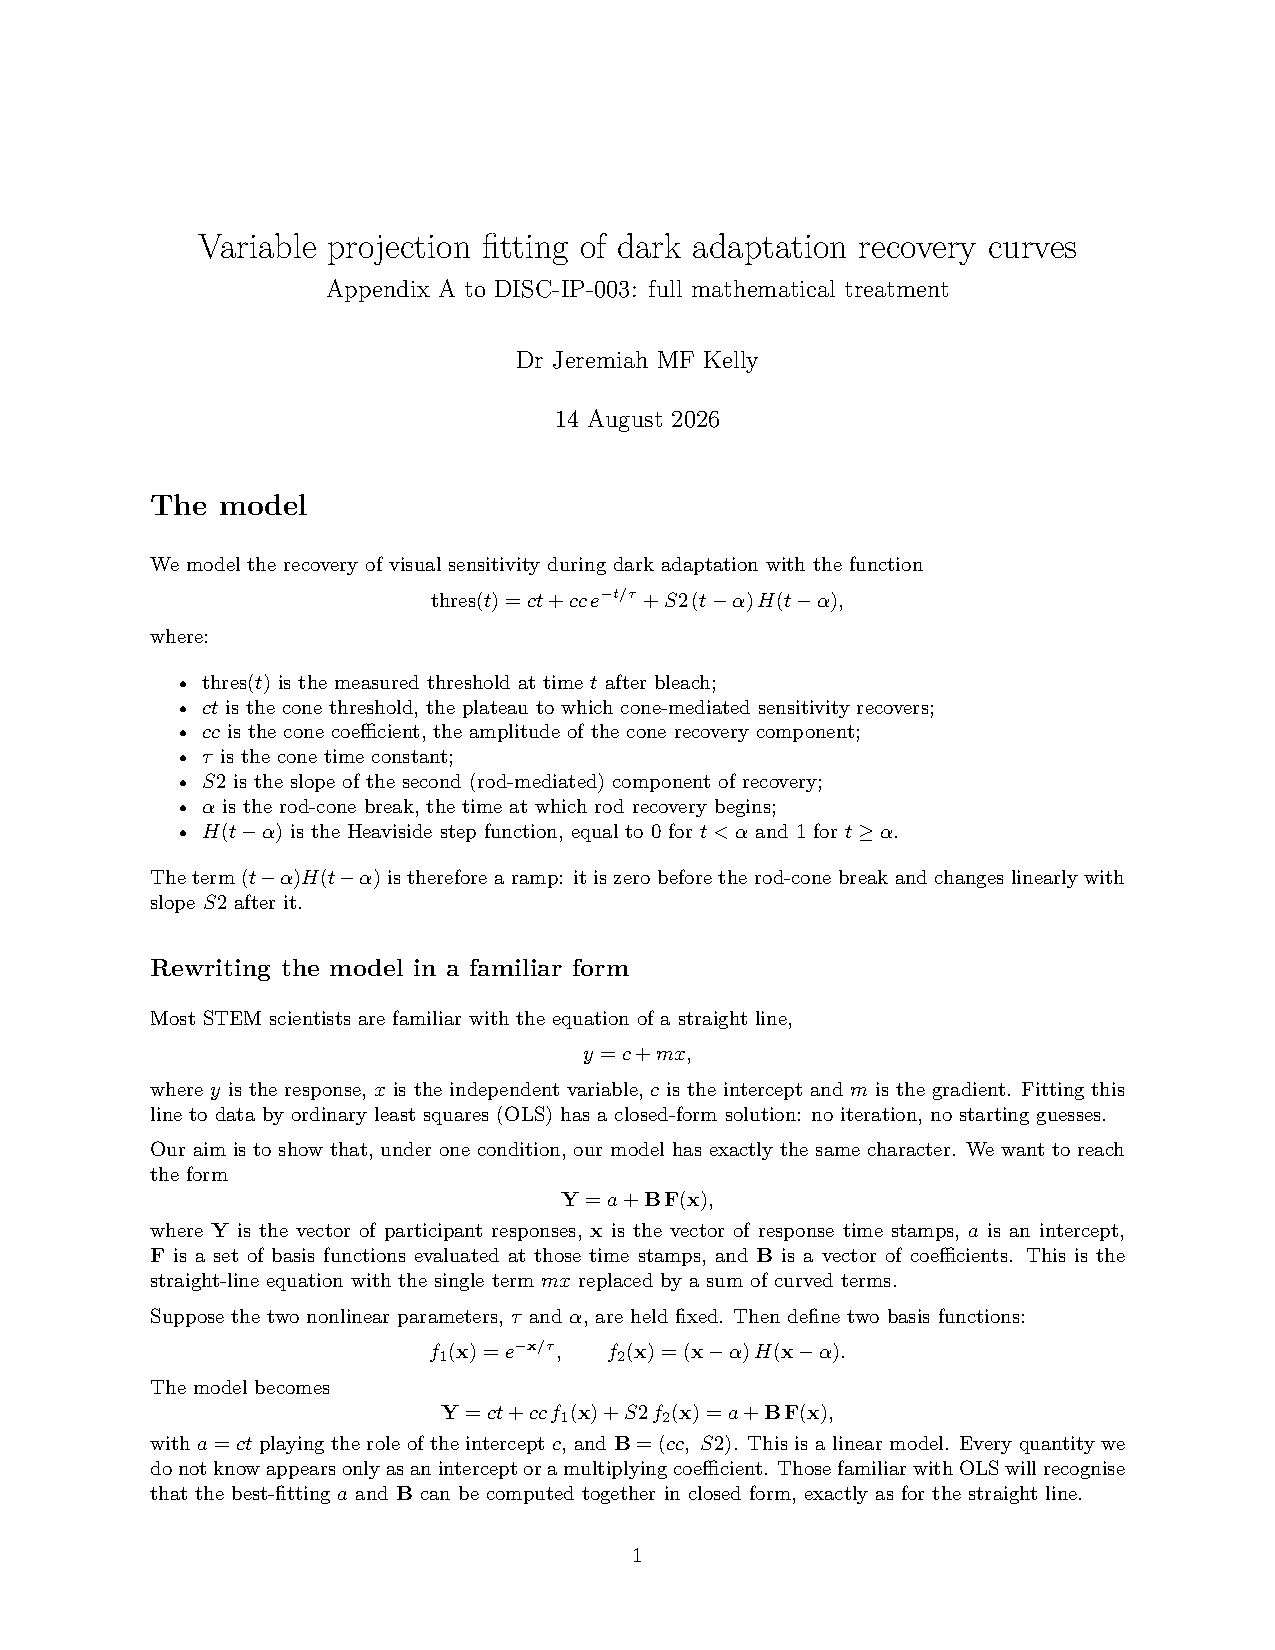
\includepdf[pages=-, pagecommand={\thispagestyle{fancy}}]{DISC-IP-003-appendix-A.pdf}%
}{%
\begin{todo}
Knit \texttt{DISC-IP-003-appendix-A.Rmd} to PDF and place
\texttt{DISC-IP-003-appendix-A.pdf} alongside this file; it will be
included here automatically on the next compile.
\end{todo}%
}

\section{Repository commit history}
Commit history of the private implementation repository, oldest first,
generated with \texttt{git log -{}-reverse -{}-date=iso} and reproduced
on 19~August~2026. Long commit bodies are abridged to their first line;
the full log is available on request.
\begin{small}
\begin{verbatim}
2026-08-03 15:29:40 +0100  420e41a  first commit
2026-08-03 20:35:36 +0100  bcb8617  Initial commit
2026-08-05 21:49:25 +0100  7b19a8d  Initial commit
2026-08-06 00:12:35 +0100  dd5ea31  Introduce profile least-squares
                                    initialisation for P5c optimisation
2026-08-06 00:15:25 +0100  cd993fd  final comment 2026-08-06
2026-08-06 11:20:39 +0100  4ca5e79  Add discrimination and inference
                                    framework
2026-08-06 12:31:21 +0100  f755c3e  simplified function to fit
                                    exponentail decay via profiled
                                    least squares
2026-08-06 12:32:04 +0100  ba96f60  minor alterations to code base in
                                    preparation for the discrimantion
                                    study
2026-08-14 01:19:25 +0100  18b12ab  Refine profiled least-squares fit
                                    for P5c model; update references
2026-08-14 01:19:25 +0100  fb67d37  Add repo plan, resources,
                                    commit-history export, and gitignore
2026-08-14 01:21:22 +0100  9cbe804  Remove editor scratch and autosave
                                    files
2026-08-15 17:26:18 +0100  bb98999  Checkpoint profiled P5c numerical
                                    experiment pipeline
2026-08-16 12:40:45 +0100  48a3a9c  Refine profile-first P5c experiment
                                    pipeline
2026-08-16 13:06:19 +0100  ef910d0  Reorganise project documentation and
                                    remove obsolete files
2026-08-18 15:38:01 +0100  9ce4a60  new refs added
2026-08-18 15:38:31 +0100  94b0c5e  new notes added
2026-08-18 15:40:43 +0100  5bb3cf4  new code updates see headers
2026-08-18 21:17:08 +0100  012d73e  CLI version that accesses Git
                                    commit code
\end{verbatim}
\end{small}
Commit messages are reproduced exactly as written, including original
spellings. Author timestamps are self-recorded; GitHub's server-side
records can corroborate them if required.

The history corroborates the account given in Section~8. The profiled
method appears at \texttt{dd5ea31} (6~August~2026), whose message records
the recognition of the partially linear structure of the model and the
replacement of a five-dimensional grid search with profiled
least-squares. The discrimination and inference framework follows the
same day. The experiment pipeline is consolidated at \texttt{bb98999}
(15~August~2026) and refined at \texttt{48a3a9c} (16~August~2026), the
latter recording that gradient refinement is skipped at profile
boundaries and that provenance is carried with each simulated result.
The final two commits, \texttt{5bb3cf4} and \texttt{012d73e}
(18~August~2026), carry the correction to the treatment of fits at the
slope bounds and the change that records the repository commit with each
experiment run. The validation experiment reported in Section~8.1 was
executed under \texttt{012d73e}.

\end{document}